\documentclass{article}
\usepackage[utf8]{inputenc}
\usepackage{todonotes}
\usepackage{array}

\title{CSC470: Software Engineering Final Report\\ TESS: The Extraordinary Sudoku Solver}
\author{Team: \#1 \\David Koval and Joseph Mammo\\Instructor: Dr. Ahyoung Lee}
\date{ 4/24/17 \\ v1.1 }

 
\renewcommand*\contentsname{Table of Contents}

 
\begin{document}
 
\maketitle

\clearpage

\tableofcontents

\clearpage

\section{Summary} 
\todo{!!!} High level summar with 1 page. the project goals, motivation or problem issues (requirements). Design considerations and choices to solve the problems to achieve the goals. Implementation, validation and testing plans.


 
\section{Introduction}
 
Overall introduction
\subsection{Purpose}
\subsection{Scope}
\subsection{Definitions, acronyms, and abbreviations}

\begin{tabular}{ | m{8em} | m{24em}|  } 
\hline
\textbf{Term}& \textbf{Definition}  \\ 
\hline
DESC & Description  \\ 
\hline
ID & Identification  \\ 
\hline
\end{tabular}

 

\section{Goals}

This is the goals section. 


 
\section{Specific Requirements}
This is the specific requirements section.

Be sure to include numbering scheme including Identifier (RQ1, RQ2, and RQn) and PW (the priority weights, may be the highest priority = 5 and the lowest priority = 1) to allow traceability.

Provide a high-level use case diagram for the high-level system models and a traceability matrix for the requirement validation.
 
\subsection{Functional Requirements}

\textbf{ID:R1} \newline TITLE: Play Game \newline DESC: The user first opens up the app, they should be able to choose the option to play a Sudoku puzzle. \newline
\textbf{ID:R2} \newline TITLE: Select Difficulty \newline DESC: The user should be able to select a difficulty setting that better suites needs at any time.
\textbf{ID:R3} \newline TITLE: Back Option \newline DESC: The user should be able to return to the main screen from the select difficulty screen if they don't select a difficulty.\newline
\textbf{ID:R4} \newline TITLE: Continue Game \newline DESC: The user should be able to continue a game that has been previously started whether or not the app has been closed. \newline 
\textbf{ID:R5} \newline TITLE:Get Puzzle \newline DESC: When the user selects a difficulty, 


\subsection{Non-Functional Requirements} 
This is the non-functional requirements section.




\section{System Design}
This is the system design section.

\subsection{Desgin Overview}
Provide an overview of the design, including diagrams, key design subsections, and how they relate or connect to one another (e.g., Interaction, structural models).

\subsection{Realistic Constraints and Professional Standards}
Identify and discuss realistic constraints on the problem, such that constraints may include economic, environmental, social, ethical, health and safety, manufacturability, policy issues, etc.

\begin{figure*}[!t]\centering
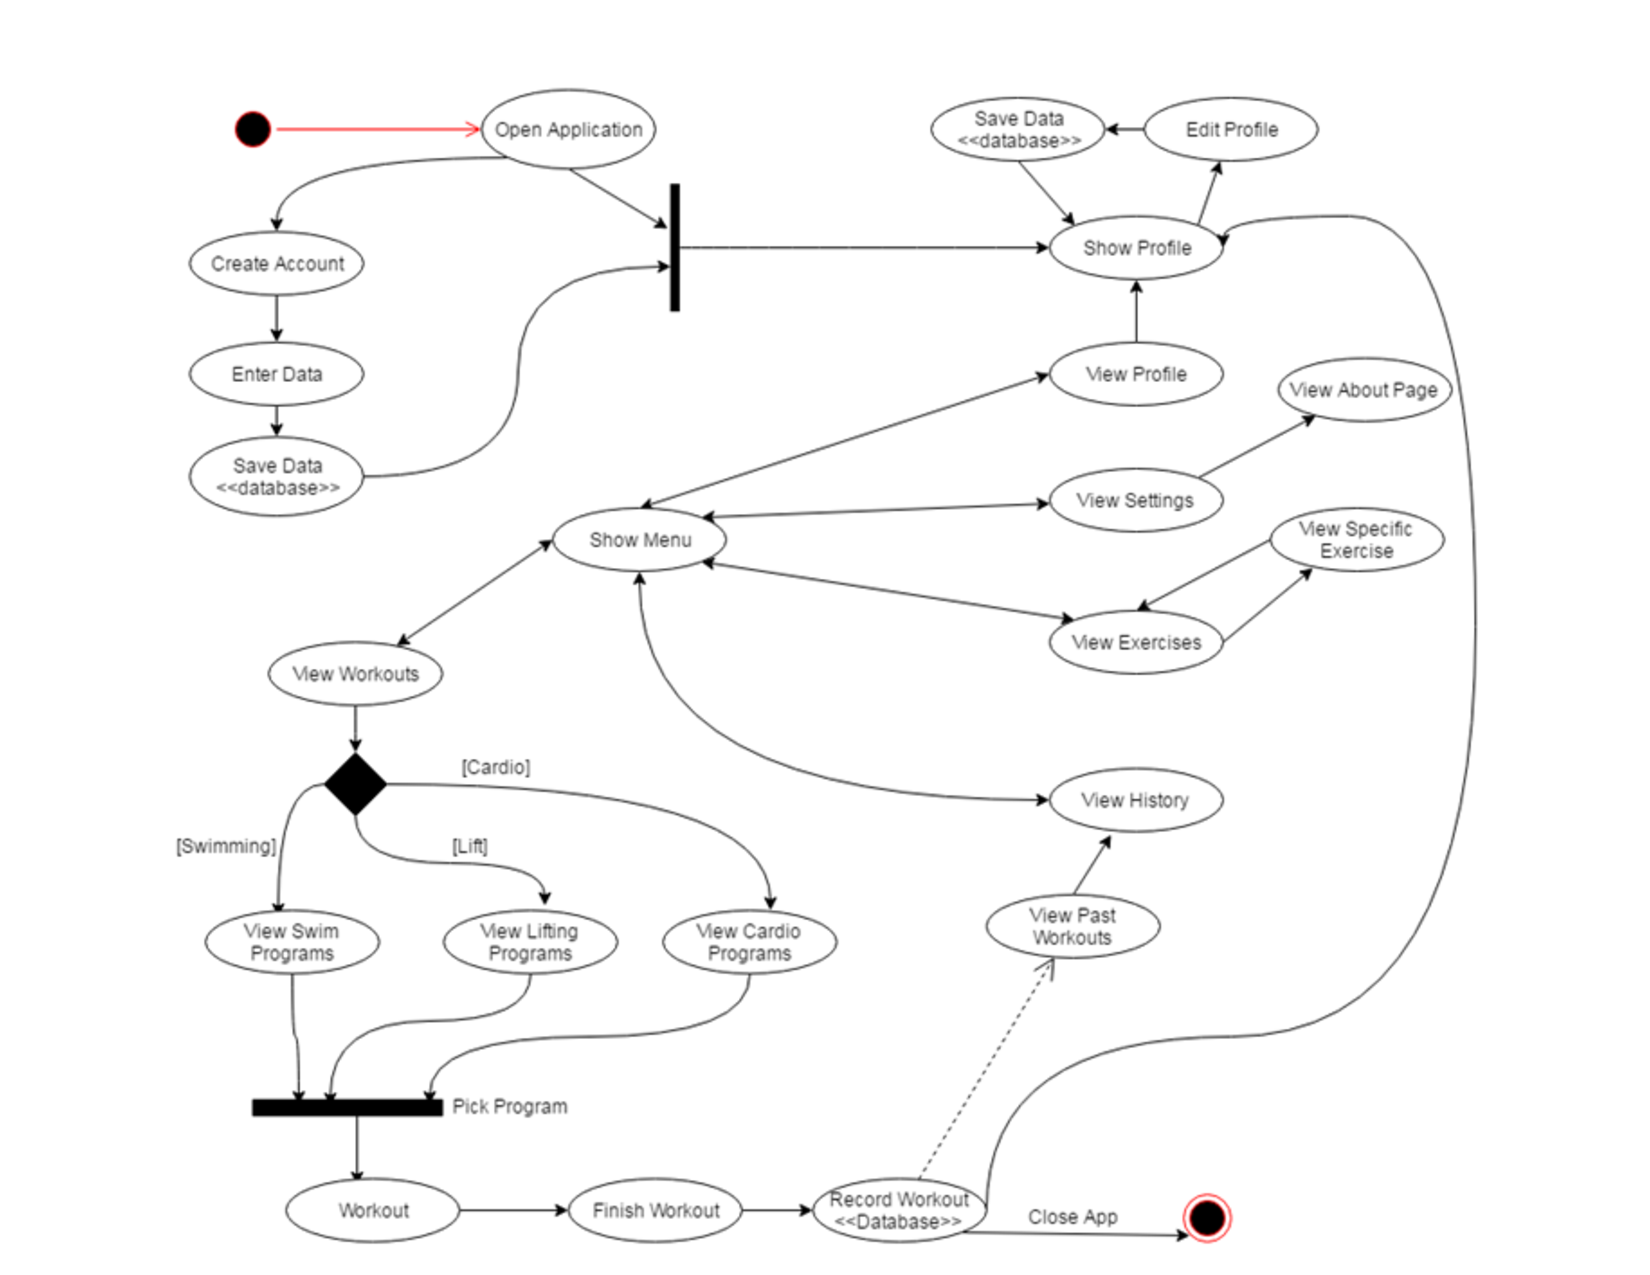
\includegraphics[width=5.0in]{./Figure/ativity.pdf}
\caption{Activity diagram of a system.}\label{fig:act_dia_1}
\end{figure*}

\subsection{Alternative Designs and Design Choices}
Describe alternative designs that were considered during execution of the project. Discuss how design choices were guided by constraints and other factors. E.g., architectural design models – Layered or Client-server and details shown using activity diagram as shown in Figure \ref{fig:act_dia_1} (Context model), sequence diagram (Interaction model), class diagram (Structural model).



\section{System Implementation}
This is the system inplementation section.

Describe the technical details for each of the subsystems or a the system-level and
provide sequence diagrams or station/activity diagrams for your system implemenation.



\section{System Testing}
This is the system testing section.

\subsection{Test Plan}
Provide your test plan with unit testing (Black-box testing and White-box testing), integration testing (Top-down or bottom-up approach) and system testing.

\subsection{Test Results}
Show your test restults and evaluate them. 

\section{Conclusions}
This is the conclusions section.

Overall summary of design methodologies, key creative approaches and potential
contribution/impact. \cite{akyildiz2014roadmap}

\bibliographystyle{IEEEtran}
\bibliography{Bibliography}


 
\end{document}